{\centering \nonumsubsection{B \hspace{1em} 组}}
\begin{xiaotis}
\setcounter{cntxiaoti}{16}
\begin{enhancedline}

\xiaoti{斜三棱柱的一个侧面的面积等于 $S$,这个侧面与它所对的棱的距离等于 $a$。求证:这个棱柱的体积等于 $\exdfrac{1}{2} Sa$。}

\xiaoti{图中长方体 $AC'$ 表示一个封闭的水箱。 已知:$BB' = 50$ cm,$AB = 70$ cm, $BC = 40$ cm。
    因为使用过久,在 $BB'$、$CC'$ 和 $AB$ 棱上各有一个小孔 $P$、$Q'$、$R$,已量得 $BR = 30$ cm,
    $BP = 20$ cm,$CQ' = 10$ cm。 如果水箱可以任意放置,那么最多能盛多少水?
}

\begin{figure}[htbp]
    \centering
    \begin{minipage}[b]{7cm}
        \centering
        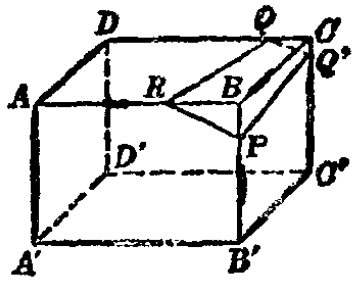
\includegraphics[width=5cm]{../pic/ltjh-ch2-fuxi-18.png}
        \caption*{(第 18 题)}
    \end{minipage}
    \qquad
    \begin{minipage}[b]{7cm}
        \centering
        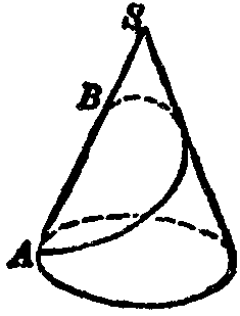
\includegraphics[width=3cm]{../pic/ltjh-ch2-fuxi-20.png}
        \caption*{(第 20 题)}
    \end{minipage}
\end{figure}


\xiaoti{一个棱锥的体积是 $V$,把棱锥的高三等分,过两个分点的平行于底面的截面将这个棱锥分成三部分。求中间一部分的体积。}

\xiaoti{有一个圆锥如图。 它的底面半径为 $r$,母线长为 $l$,且 $l > 2r$,在母线 $SA$ 上有一点$B$,$AB = a$。
    求由 $A$ 绕圆锥一周到 $B$ 的最短距离是多少?
}

\xiaoti{如果正四棱锥的侧面是正三角形,求证:它的相邻两个侧面所成的二面角,是侧面和底面所成二面角的二倍。}

\xiaoti{一个外径是 12 cm,壁厚为 0.2 cm 的钢球,能否浮在水面上(钢的比重是 $7.8\;\kmlflm$)?}

\xiaoti{边长为 $a$ 的正六边形,以它的一边为轴旋转,求旋转体的全面积和体积。}

\end{enhancedline}
\end{xiaotis}
